%%%%%%%%%%%%%%%%%%%%%%%%%%%%%%%%%%%%%%%%%%%%%%%%%%%%%%%
% Math 3250 Combinatorics, University of Connecticut
%%%%%%%%%%%%%%%%%%%%%%%%%%%%%%%%%%%%%%%%%%%%%%%%%%%%%%%

% Anything after a percent sign is a comment.

% Necessary first line. \documentclass defines the type of document and some options (for example, try changing the font size (10pt or 11pt or 12pt).
\documentclass[10pt]{amsart}
\usepackage{enumerate} % to be able to enumerate a list using non-numbers
\usepackage{tikz}
%for hypertext references
\usepackage[colorlinks = true,
            linkcolor = blue,
            urlcolor  = blue,
            citecolor = red,
            anchorcolor = green]{hyperref}


\usepackage[letterpaper]{geometry} 
\geometry{tmargin=0.3in,bmargin=0.2in,lmargin=0.50in,rmargin=0.50in}
\voffset -0.0in


\begin{document}

\begin{center}\textbf{Math3250 Combinatorics Reading HW 16}\end{center}

% --------------------------------------------------------
%                         Start here
% --------------------------------------------------------



\subsection*{Instruction}

\begin{itemize}
\item 
Submit your homework by email (subject: Math3250 Combinatorics Reading HW 16). Either hand-write (use a scanner app to convert to PDF) or type your work.
\item
Ref: textbook \emph{Combinatorics and Graph Theory} by Harris, Hirst, and Mossinghoff (HHM) Sec 1.3
\end{itemize}





\section{Sec 1.3.4 Counting trees}
Either watch the lecture video of Sec 1.3.4 Counting trees (25 minutes) or read Sec 1.3.4 from \href{https://egunawan.github.io/combinatorics/notes/notes1_3trees.pdf}{lecture notes for Sec 1.3 video on trees}. 
Write down what you did. If you watched the video, please specify (Kaltura/YouTube) and type of device. The video is at original speed --- you can play the video at faster speed if you are not taking notes.


\section{Exercises}

\begin{enumerate}[a.)]
	
\item 
Determine the Pr\"{u}fer sequence for each of the two trees below.

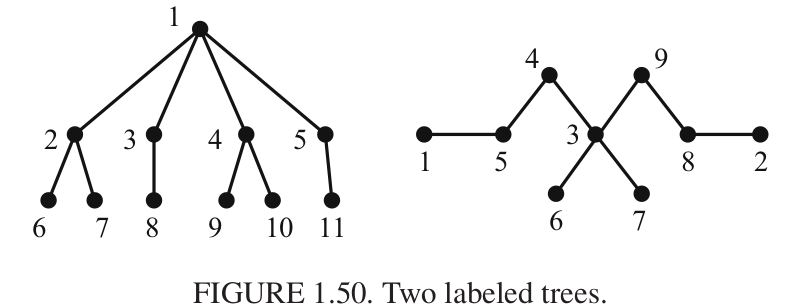
\includegraphics[width=2.8in]{reading16.png}

\bigskip
	
\item 
Draw and label a tree whose Pr\"{u}fer sequence is $5, 4, 3, 5, 4, 3, 5, 4, 3.$

\bigskip
	
\item 
Which trees have constant Pr\"{u}fer sequence? 
What trees have Pr\"{u}fer sequences with distinct terms?

\bigskip

\item 
(Optional) Read the following. 	\\
Recall from Linear Algebra that the following matrix operation does not change the determinant of a matrix: replacing row $i$ with the sum of row $i$ and row $j$.
	
	
We will use the Matrix Tree Theorem to prove that the number of spanning trees of the labeled tree $K_5$ is $5^3$. 
First, we compute $D-A$.
\begin{equation*}
D=\begin{bmatrix}
4 & 0 & 0 & 0 & 0\\
0 & 4 & 0 & 0 & 0\\
0 & 0 & 4 & 0 & 0\\
0 & 0 & 0 & 4 & 0\\
0 & 0 & 0 & 0 & 4\\
\end{bmatrix},
~~
A=\begin{bmatrix}
0 & 1 & 1 & 1 & 1\\
1 & 0 & 1 & 1 & 1\\
1 & 1 & 0 & 1 & 1\\
1 & 1 & 1 & 0 & 1\\
1 & 1 & 1 & 1 & 0\\
\end{bmatrix},
~~
D-A=\begin{bmatrix}
4 & -1 & -1 & -1 & -1\\
-1 & 4 & -1 & -1 & -1\\
-1 & -1 & 4 & -1 & -1\\
-1 & -1 & -1 & 4 & -1\\
-1 & -1 & -1 & -1 & 4\\
\end{bmatrix}
\end{equation*}

Let $M=D-A$. 
The $1,1$ cofactor of $M$ is  $(-1)^{1+1} det(M(1\mid 1))$. 

\begin{equation*}
M(1 \mid 1) = 
\begin{bmatrix}
4 & -1 & -1 & -1 \\
-1 & 4 & -1 & -1 \\
-1 & -1 & 4 & -1 \\
-1 & -1 & -1 & 4 \\
\end{bmatrix}.
\end{equation*}

To simplify the computation of $det(M(1\mid 1))$, we will perform matrix operation which does not alter the value of the determinant. 
First, replace the first row with the sum of all rows. We get
\begin{equation*}
\begin{bmatrix}
1 & 1 & 1 & 1 \\
-1 & 4 & -1 & -1 \\
-1 & -1 & 4 & -1 \\
-1 & -1 & -1 & 4 \\
\end{bmatrix}.
\end{equation*}

Next, replace each row $i$ (except for the first row) with the sum of row $i$ and the first row. We get 
\begin{equation*}
\begin{bmatrix}
1 & 1 & 1 & 1 \\
0 & 5 & 0 & 0 \\
0 & 0 & 5 & 0 \\
0 & 0 & 0 & 5 \\
\end{bmatrix}.
\end{equation*}	
The determinant of the above matrix is $5 \cdot 5 \cdot 5 = 5^{3}$.

\bigskip

\item 
Use the Matrix Tree Theorem to prove Cayley's Theorem. 
(Do the above computation for a general $n$. See also Example 10.21 p. 249-250 in B\'ona's textbook.)

\end{enumerate}



	\section{Last Section}
\begin{itemize}
	\item 
	Email me with a few of the above exercises that you would like to present during class on Thurs Apr 23.
	\item
	Questions, comments, suggestions?
\end{itemize}



\end{document}
